
\chapter{Expansion of MRCs}
While MRC generation has been made efficient via Mattson's algorithm, it is limited in the use of the paging model. This research extends the efficient generation of MRCs using Mattson's algorithm to the cost model. To do this, we propose a new algorithm called Sum Cost Priority (SCP).



\section{What is SCP}
The Sum Cost Priority (SCP) caching algorithm allows for the efficient creation of MRCs in the cost model. 

SCP is a stack algorithm in the cost model. SCP works by keeping a priority of items that are currently in the cache. However, unlike LRU where the priority of an item is equal to the number of distinct items that have been accessed since its last access, SCP assigns a priority score to each item based on its access cost. Specifically, we update priority by cost rather than 1, and we update every item in the cache regardless of whether it has a higher or lower priority. When a new item is requested, SCP sets its priority to its cost and then subtracts its cost from all items in the cache. If the cache is full, the item in the cache with the lowest priority is evicted. We do this to distinguish items, as they have differing costs and need to have repeated access to the same item eventually forcing out more expensive items.




\begin{algorithm}
\caption{Sum Cost Priority}\label{euclid}
    \begin{algorithmic}[1]
        \BState \emph{loop}:
            \State $\textit{Item} \gets \text{nextItem in trace}$
            \ForEach {$f \in cache $}
                    \State $priority(f) \gets priority(f) - cost(i)$
            \EndFor
            \If {$\textit{Item}(i) \text{not in Cache}$}
                    \State $\text{Evict} \min priority(f)$
            \EndIf
            \State $priority(Item) \textbf{ }= \textbf{ }cost(Item)$
    \end{algorithmic}
\end{algorithm}





To show an algorithm is good theoretically, as described in Chapter 3, we aim to show that it has lower and upper bounds on its competitive ratio that is close to $\frac{k}{k-h+1}$.  \cite{sleator1985amortized} proved that any deterministic algorithm has this $\frac{k}{k-h+1}$ bound. This means that SCP also has this bound as it is deterministic.

For the upper bound of SCP, we currently do not have proof to show the worst-case miss ratio when compared to OPT. There has been some work done by Riley Shahar that shows that the upper bound is O($2^k$).


\section{SCP is a Stack Algorithm}
This is proof that shows, given this structure, that SCP is a stack algorithm.

\newtheorem{theorem}{Theorem}[section]
\newtheorem{corollary}{Corollary}[theorem]
\newtheorem{lemma}[theorem]{Lemma}
\newtheorem{definition}{Definition}[section]
\begin{lemma}
An SCP cache(k)$\subseteq$ cache(k+1). \\ Let
$cache(k)$ be a cache of size k and let $cache(k+1)$ be cache of size k+1 \\

\textbf{Base Case:}
Both $cache(k)$ and $cache(k+1)$ start out with empty caches as defined in the abstract caching problem. This means that until either cache makes an eviction
\[cache(k) \subseteq cache(k+1)\]
\\
\textbf{n case}
Suppose that at time t, which is a point after both caches are full, the size of items in $cache(k) = k$ and the size of items in $cache(k+1)=k+1$ and that $cache(k) \subseteq cache(k+1)$
Then access item $i_{t+1}$ at time $t+1$
This creates 3 cases:\\
\textbf{Case 1:}
\[i_{t+1} \in cache(k)\] \[cache(k) \subseteq cache(k+1)\] $i_{t+1}$ also is in cache(k+1)
Since $i_{t+1}$ exists in both caches, no evictions occur as the item is a hit on both caches

\textbf{Case 2:}
\[i_{t+1} \in cache(k+1)\text{, but } i_{t+1} \notin cache(k)\]
Since $i_{t+1}$ exists in only cache(k+1), the possible items in cache(k) at time t+1 are
\[(cache_{t}(k) \cup i_{t+1}) \subseteq cache_{t+1}(k+1)\]
as since $i \in cache(k+1)$ at time t+1, $cache(k) \cup i_{t+1}$ must equal cache(k+1) as cache(k) is a subset at time t and the only newly accessed item is $i_{t+1}$. This means that cache(k+1) does not change its eviction decisions due to cache(k) eviction decisions.  

\textbf{Case 3:}
\[i_{t+1} \notin cache(k+1), and i{t+1} \notin cache(k)\]
Since $i_{t+1}$ exists in neither cache(k+1) or cache(k) at time t, an item must be evicted from cache(k+1). \\ \\
Let $i_a$ be the minimum priority item of cache(k+1) at time t and $i_b$ be the minimum priority item of cache(k) at time t.\\
There are 2 possible cases for items $i_a$ and $i_b$, either $i_a$=$i_b$, meaning that both these items have the same priority, or $i_a \neq$ $i_b$, meaning that $i_a$ priority is not the same as $i_b$.\\

\textbf{Case 3a:}
\[i_a=i_b\]
This means there is only one possible item list for caches k and k+1 at t+1

\[cache_{t+1}(k+1) =  (cache_{t}(k+1)\cup i_{t+1}) / i_a \]
\[cache_{t+1}(k) =  (cache_{t}(k)\cup i_{t+1}) / i_b \]

by applying  
\[(cache_{t}(k) \cup i_{t+1}) \subseteq cache_{t+1}(k+1)\]
 we can show that they both evict the same item at t+1 \\

 \textbf{Case 3b:}
\[i_a \neq i_b\]
This means that $i_a \notin cache(k)$ as this would mean that $i_b$ is not the item with the least priority in as that would be contradictory. This then means that evicting $i_a$ will keep cache(k)$\subseteq$ cache(k+1) \\ \\ \\

These cases then prove that SCP is in fact a stack algorithm as cache(k)$\subseteq$ cache(k+1) no matter what items are requested $\qed$
\end{lemma}



\section{Methodology}
For our simulations, we use \cite{snia-trace-block-io-28571} and \cite{cacheWorkload-OSDI20}. These traces represent requests made to an SSD and Twitter servers. Each of these traces is analyzed over their entire length ranging from 1 to 10 million requests. Along with these two sets of traces from real systems, we generated our own to gather more data, these generated traces ranged from 1 million to 10 million requests.
On these traces, we compare SCP against Landlord. Landlord has been proven to have the $\frac{k}{k-h+1}$ bound for the cost model, meaning that it performs as best as any online algorithm can. Comparing SCP against Landlord on these traces allows us to analyze how SCP performs in real systems. We compare these two algorithms on their total cost paid over the trace when generating MRCs. This is important as in this model MRCs don't just look at the actual miss ratio on traces, they look at the total cost paid by these algorithms. This is because it can be more effective to continually evict a low-cost item than a high-cost one.

\section{SCP vs Landlord}
To demonstrate that SCP performs well in practice, we tested it against a provably good algorithm in the cost model called Landlord. These experiments showed that SCP is an effective algorithm at limiting the cost paid by caches on a trace, as on $65.07\%$ of traces it performed within $\pm 5\%$ of Landlord. 

\subsection{SNIA IOTTA Traces}
At first, when testing SCP against Landlord, we used traces from \cite{snia-trace-block-io-28571}. A stack distance histogram representing a trace can be seen in Figure 5.1. As can be seen, most items were only accessed once, with only a small percentage of requests being to previous items. This then made these traces unhelpful to comparison as because the items were accessed so infrequently, there was very little benefit of using a cache.

\begin{figure}[h]
    \centering
        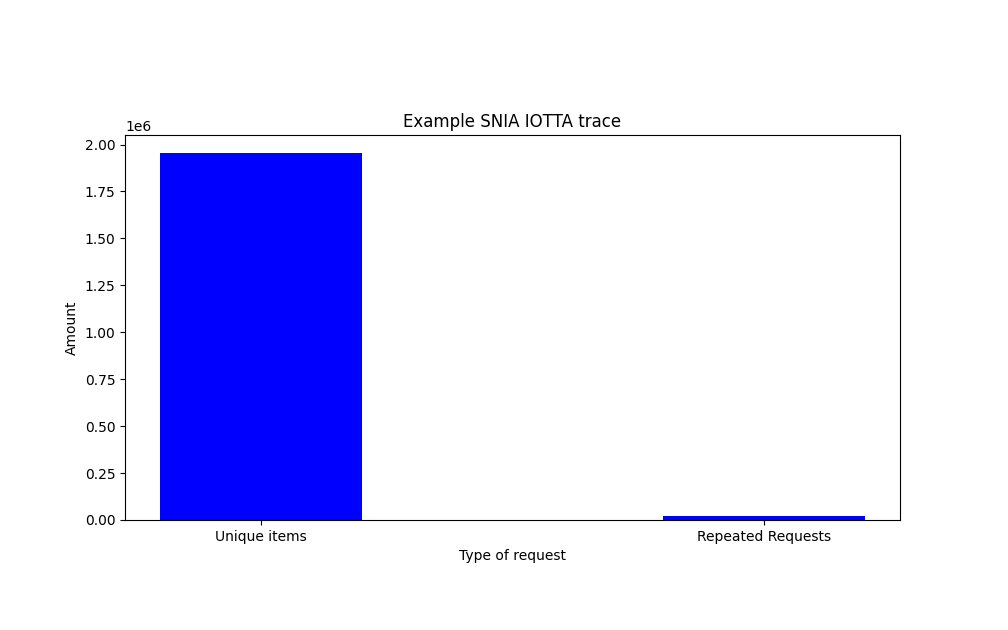
\includegraphics[scale=0.6, trim={0cm 0cm 0 0cm},clip]{thesistemplate_2020-04-24/chapters/ch5/aaaaaaaaaaaaa.png}
    \caption{Items in a SNIA IOTTA Trace}
    \label{fig:my_label}
\end{figure}


Instead of using these traces in their entirety, we instead decided to limit the number of items in a trace from \cite{snia-trace-block-io-28571}. We did this in the hope that we would get traces wherein items were accessed more frequently as there would be fewer unique items that would be accessed more frequently.

Even with this limitation, this trace generated an MRC that had the total cost paid for both Landlord and SCP so large that there was not a meaningful comparison to be made on any cache size. We then decided to not continue using these traces because of their structure. 



\subsection{Twitter Traces}
These SNIA IOTTA traces that were tested were not promising, so we sought to find traces of systems that would not suffer from the same problems of item accesses. After some searching, we found a set of traces from \cite{cacheWorkload-OSDI20} that showed some promise. Figure 5.2 shows how SCP performed versus Landlord on one of the traces provided by Twitter. As can be seen, quite clearly, these traces did not suffer the same issues as the traces from SNIA IOTTA. We chose this specific trace to show in this figure as it shows that SCP consistently pays 3\% less than Landlord on caches from size 10,000 to 100,000.


This increase in performance over Landlord was not limited to this trace though. On 82.1\% of these traces, SCP was performing within $\pm 5\%$ of Landlord. 

\begin{figure}[h]
  \begin{center}
    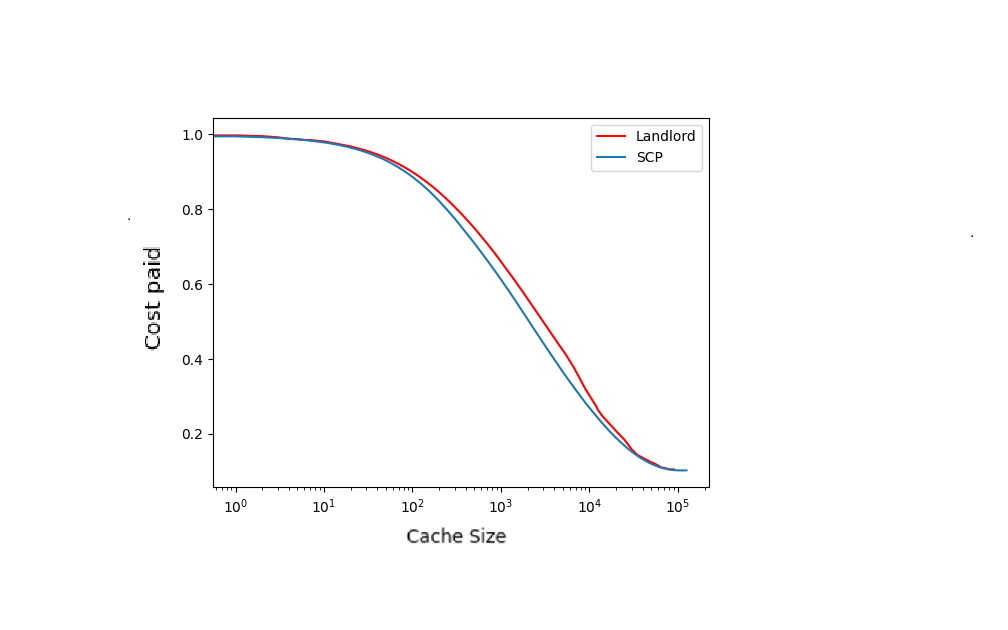
\includegraphics[scale=.5,trim={2cm 2cm 0 2cm},clip]{thesistemplate_2020-04-24/chapters/ch5/SCPresul.png}
  \end{center}
  \caption{SCPs performance vs Landlord on a Twitter trace}
\end{figure}


\subsection{Generated Traces}
With these results of the traces so far, instead of using real-world traces, we generated our own set of traces as more data points to check SCPs performance against. We generated these data to look at what happens to SCPs comparative performance to Landlord when costs either varied slightly, greatly, or not much and what happens when we vary how often items occur together.


In general, as shown in Figure 5.3, which is a sample of a generated trace, it can be seen that SCP performs almost identically to Landlord on all cache sizes. These are great results because it founds a reasonable hope that SCP will perform well as a cache algorithm in a variety of circumstances. In fact, in these traces, SCP performs $\pm 5\%$ of Landlord on $62.3\%$ of traces.


\begin{figure}[H]
    \centering
    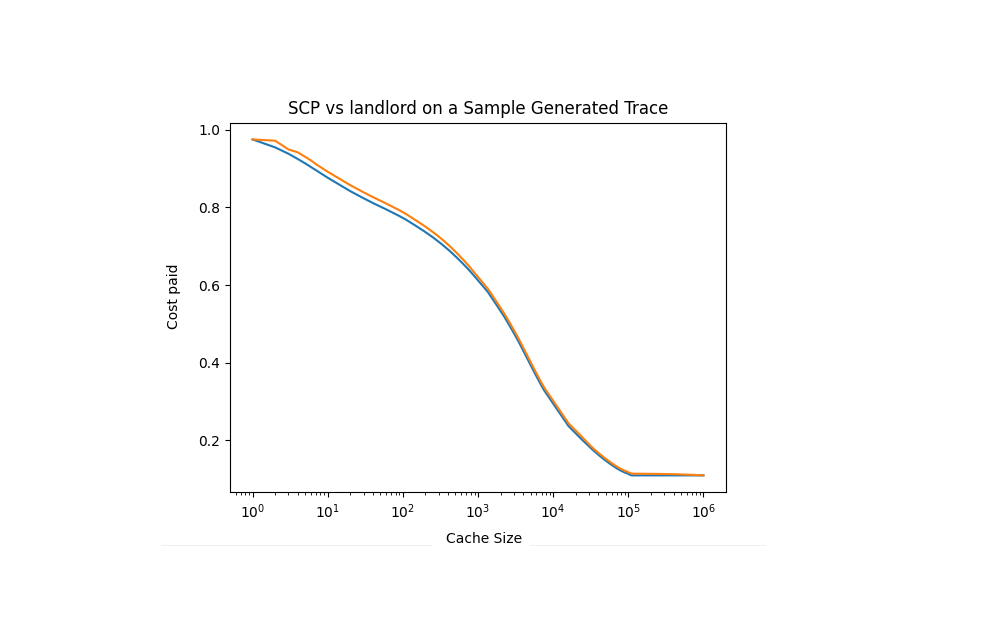
\includegraphics[scale=.6,trim={2cm 1cm 2cm 1cm},clip]{thesistemplate_2020-04-24/chapters/ch5/GenTrace.png}
    \caption{SCP's performance on a sample generated trace}
    \label{fig:my_label}
\end{figure}

\subsection{Aggregated Results}
After analyzing the traces that we gathered, both from Twitter and the generated traces, we wanted to understand how SCP performed against Landlord in total paid cost over all caches in all tested traces. This data is then shown in Figure 5.5. The positive variance is where SCP performs better than Landlord and the negative is where it performs worse. To create this graph, we normalized the cost paid on a trace to Landlord's paid cost, then found how much SCP varied from it. We did this for all cache sizes we had data for and compared them.

\begin{figure}[ht]
  \begin{center}
    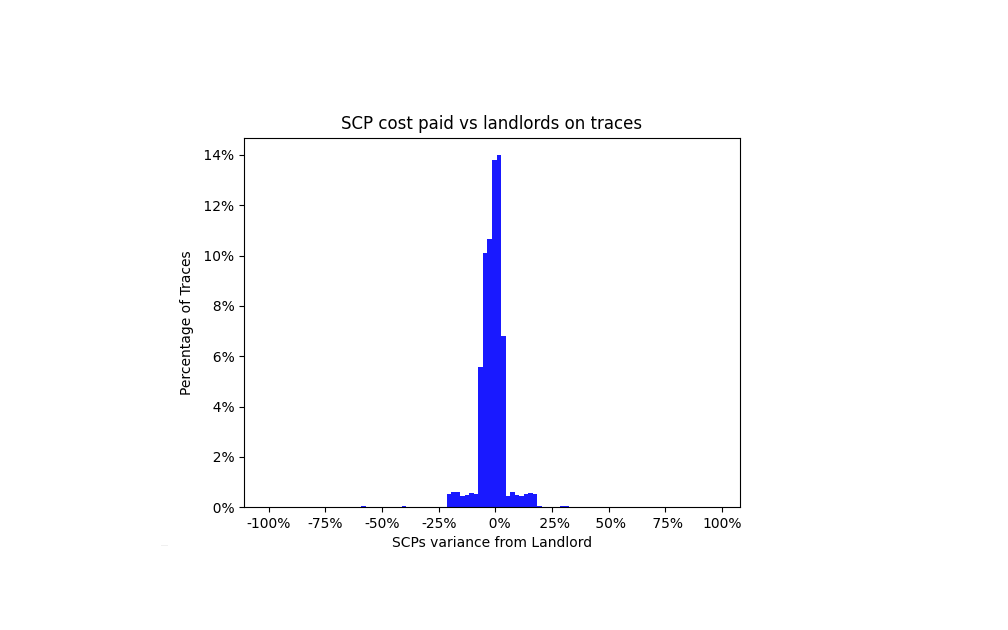
\includegraphics[scale=.6,trim={0 2cm 0 3cm},clip]{thesistemplate_2020-04-24/chapters/ch5/histFin.png}
  \end{center}
  \caption{SCP's performance over many traces}
\end{figure}


We see in Figure 5.4 that SCP performs within 5\% of Landlord 65.07\% of the time, within 25\% of landlord 99.72\% of the time, with only 0.28\% of caches performing worse than 25\%.

These results are incredibly promising and show that SCP performs well against Landlord in a variety of traces.